% simdoc.tex V3.0, 30 March 2010

\documentclass[times]{simauth}

\usepackage{moreverb}

%\usepackage[T1,mtbold]{mathtime} % commented by ShareLaTeX Team because of compilation errors

\usepackage[
%dvips, % commented by ShareLaTeX Team because of compilation errors
colorlinks,bookmarksopen,bookmarksnumbered,citecolor=red,urlcolor=red]{hyperref}

\usepackage[utf8]{inputenc}
\usepackage[T1]{fontenc}
\usepackage[spanish]{babel}
\usepackage{wrapfig}
\usepackage{framed}
\usepackage{upquote}
\usepackage{epigraph}
\usepackage{makeidx}
\usepackage{pdfpages}
\graphicspath{ {images/} }

%\newcommand{\mysmall}{\fontsize{7.5pt}{8pt}\selectfont}

%\newcommand\BibTeX{{\rmfamily B\kern-.05em \textsc{i\kern-.025em b}\kern-.08em
%T\kern-.1667em\lower.7ex\hbox{E}\kern-.125emX}}

\def\volumeyear{2010}

\begin{document}

%\runninghead{A.~N.~Other}

\title{
    {\fontfamily{ppl} \fontsize{30}{1} \selectfont{
        Tarea \#3:\\ Falacias de razonamiento en medios de comunicación nacional}
    }
}

\author{
    {\fontfamily{ppl} \fontsize{14}{1} \selectfont{
        Carlos Martín Flores González \\
        Raquel Rodríguez Chaves}
    }
}

%\address{John Wiley \& Sons, Ltd, The Atrium, Southern Gate, Chichester,
%West Sussex, PO19~8SQ, UK}
%
%\corraddr{Journals Production Department, John Wiley \& Sons, Ltd,
%The Atrium, Southern Gate, Chichester, West Sussex, PO19~8SQ, UK.}

%\begin{abstract}
%This paper describes the use of the \LaTeXe\ \textsf{simauth.cls}
%class file for setting papers for \emph{Statistics in Medicine}.
%\end{abstract}

%\keywords{class file; \LaTeXe; \emph{Statist.\ Med.}}

\maketitle

\tableofcontents

\newpage
\section{Falacia 1: Diputado equipara Costa Rica con la Alemania Nazi}

\begin{figure}[h]
    \centering
    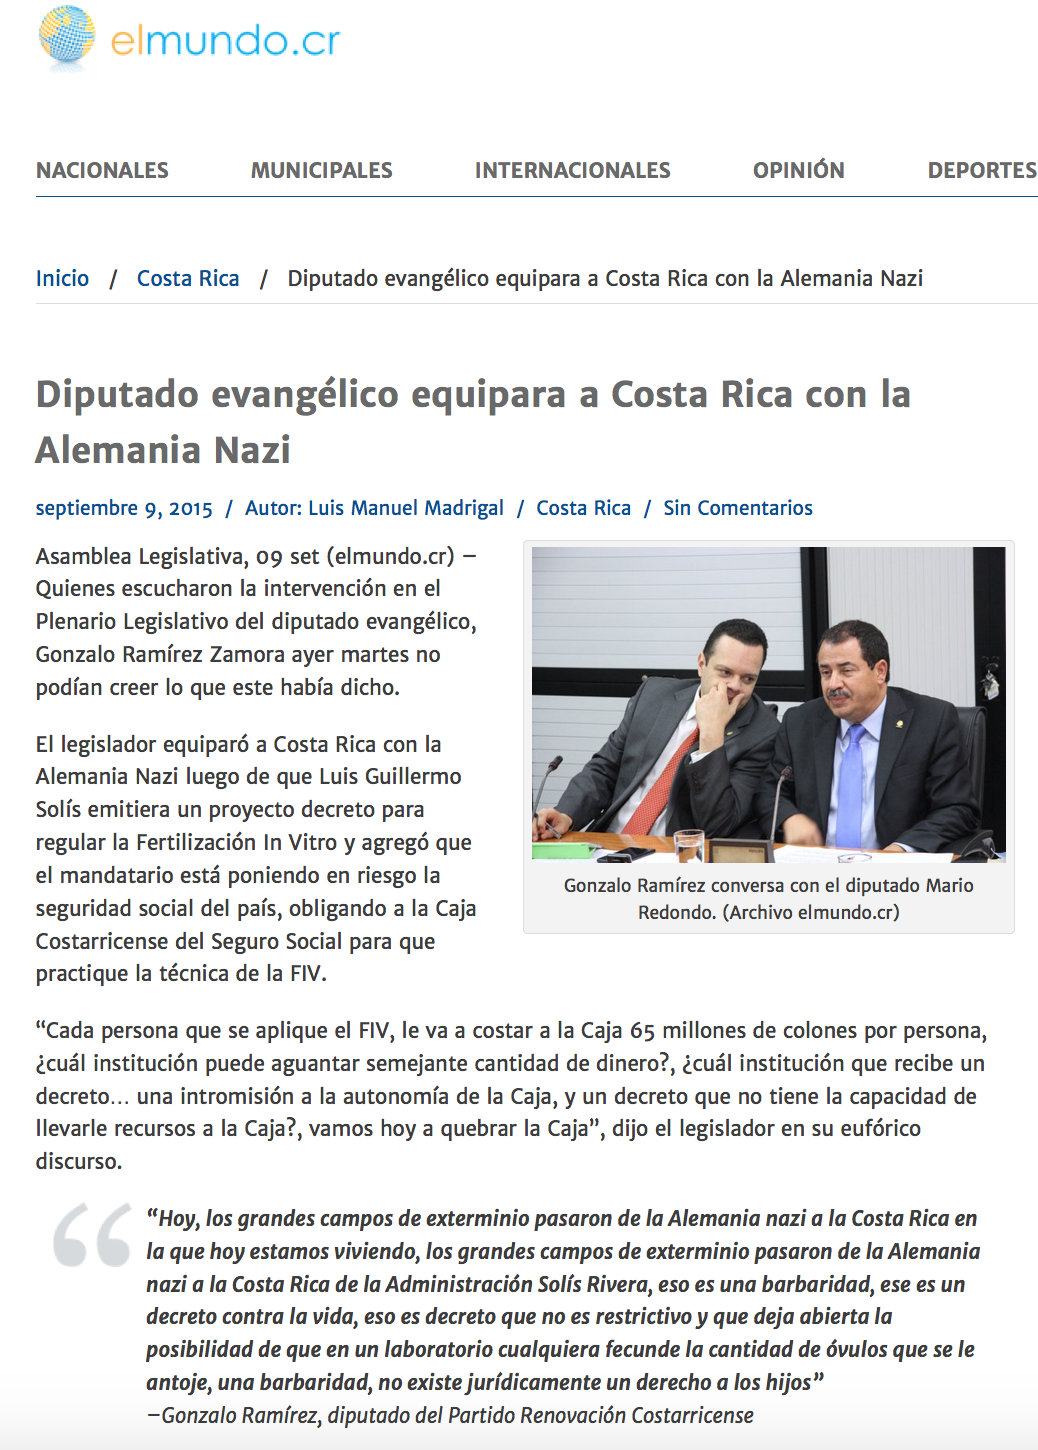
\includegraphics[width=15cm]{costarica-nazi-fiv}
    \captionof{figure}{Captura de pantalla de la noticia}
    \label{fig:falacia1}
\end{figure}

\newpage

\begin{table}[h!]
    \begin{tabular}{ll} 
        \toprule[1.5pt]
        Fuente & Periódico \href{http://elmundo.cr}{elmundo.cr}\\
        \midrule[0.5pt]
        Fecha  & 9 de setiembre 2015\\
        \midrule[0.5pt]
        Falacia & Palabras emotivas \\
        \bottomrule[1.5pt]
    \end{tabular} 
\end{table}

El legalización de la técnica de Fertilización in Vitro (FIV) ha resultado ser un tema muy polémico en nuestro país, principalmente en la asamblea legislativa en donde un pequeño grupo de diputados de partidos conservadores se oponen a la utilización de esta técnica aduciendo que atenta contra la vida humana.

En su discurso de la sesión del día martes 8 de setiembre del 2015, el diputado evangélico Gonzalo Ramírez Zamora, un claro opositor del FIV, llegó a comparar a Costa Rica con la Alamania Nazi diciendo que: \textit{``Hoy, los grandes campos de exterminio pasaron de la Alemania nazi a la Costa Rica en la que hoy estamos viviendo, los grandes campos de exterminio pasaron de la Alemania nazi a la Costa Rica de la Administración Solís Rivera, eso es una barbaridad, ese es un decreto contra la vida, eso es decreto que no es restrictivo y que deja abierta la posibilidad de que en un laboratorio cualquiera fecunde la cantidad de óvulos que se le antoje, una barbaridad, no existe jurídicamente un derecho a los hijos''}.

En su discurso el diputado Ramírez hace un claro uso de palabras emotivas con el fin de despertar sentimientos negativos ante la posible aprobación de esta técnica, de esta forma tanto diputados presentes, seguidores de su partido y público en general podrían llegar a crear sentimientos de miedo u odio con el fin de generar mayor oposición.

\noindent Dirección: \href{http://www.elmundo.cr/costarica/diputado-equipara-costa-rica-la-alemania-nazi-decreto-la-fiv/}{http://www.elmundo.cr/costarica/diputado-equipara-costa-rica-la-alemania-nazi-decreto-la-fiv/} \\
Discurso del diputado Ramírez: \href{https://www.youtube.com/watch?v=cK6AeaFB1Co}{https://www.youtube.com/watch?v=cK6AeaFB1Co}\\


\newpage
\section{Falacia 2: Periodistas cuestionan a la costarricense del milagro sobre los incrédulos}

\begin{figure}[h]
    \centering
    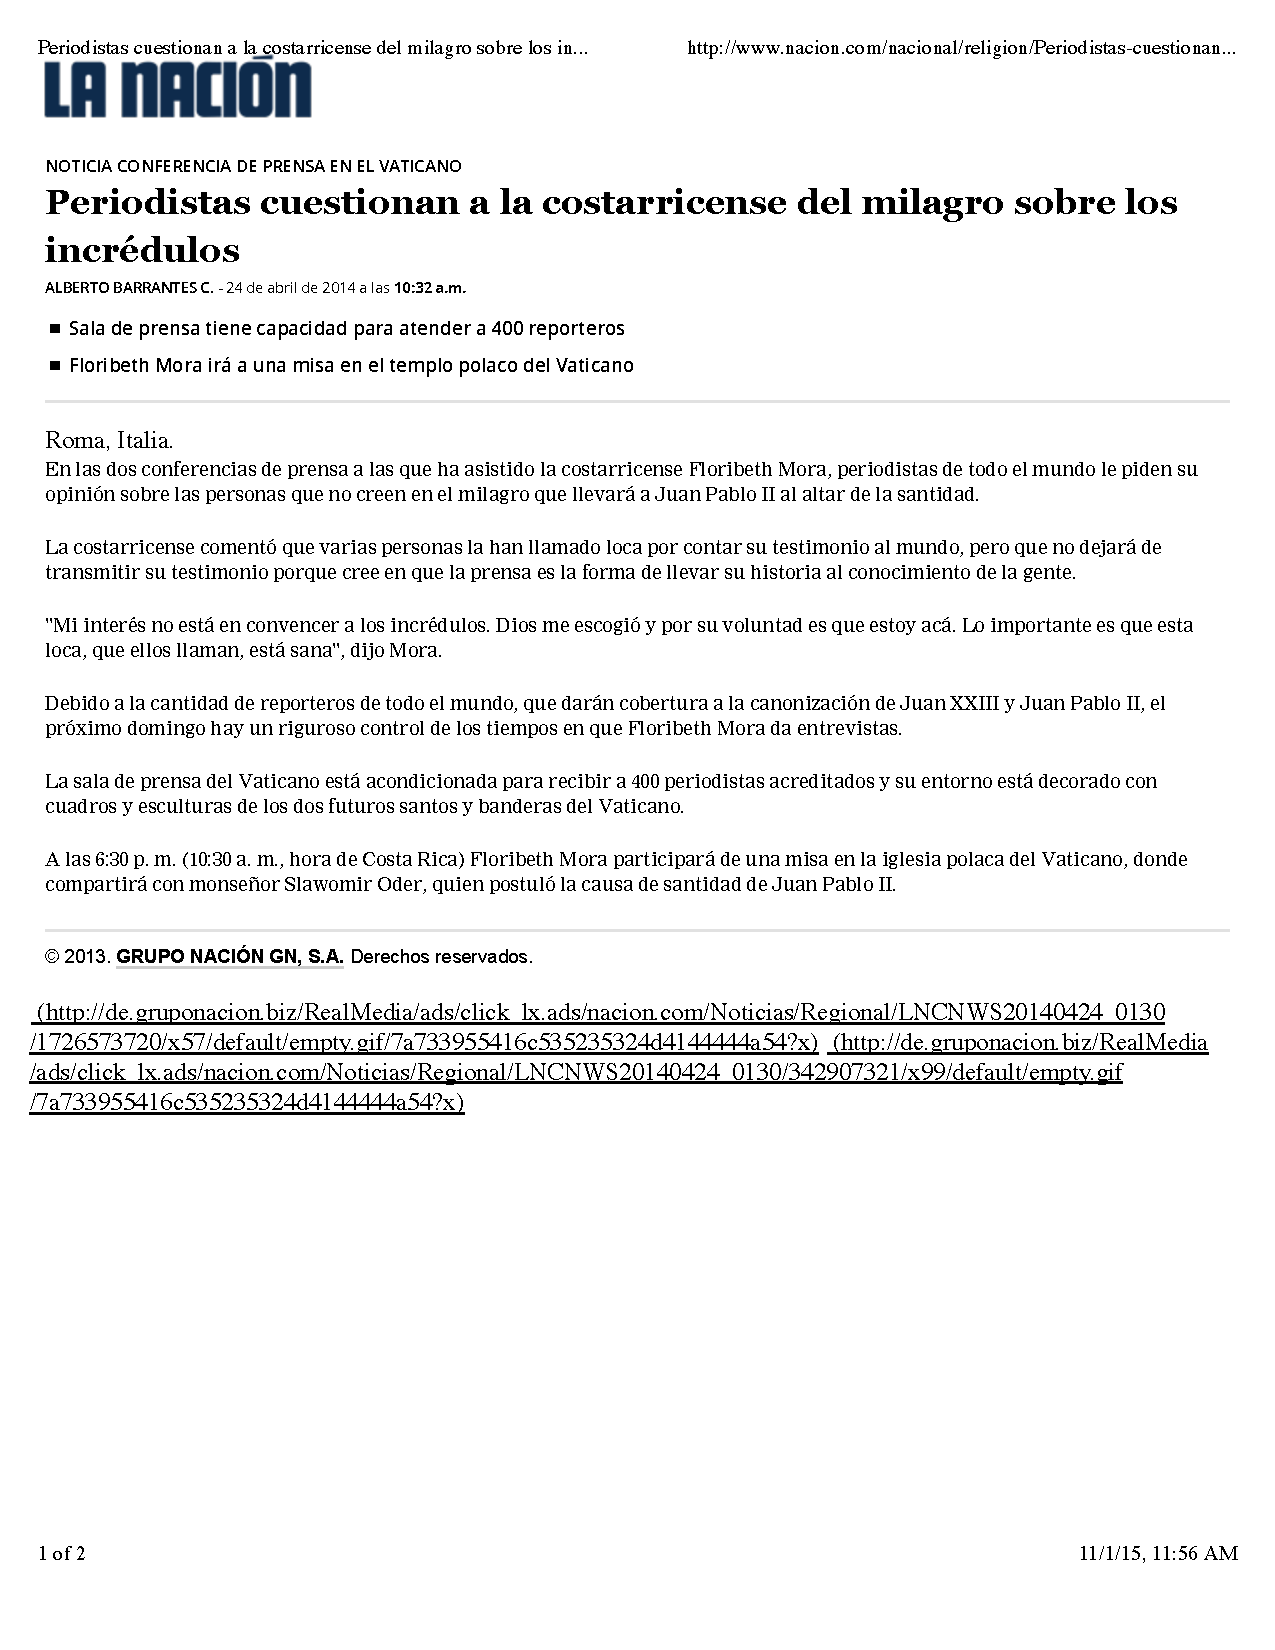
\includegraphics[width=15cm]{floribeth-mora-milagro}
    \captionof{figure}{Detalle de la noticia sobre el cuestionamiento del milagro de Floribeth Mora}
    \label{fig:falacia2}
\end{figure}

\newpage

\begin{table}[h!]
    \begin{tabular}{ll} 
        \toprule[1.5pt]
        Fuente & Periódico La Nación\\
        \midrule[0.5pt]
        Fecha  & 24 de abril 2014\\
        \midrule[0.5pt]
        Falacia & Peso de la prueba, Inexplicado vs Inexplicable \\
        \bottomrule[1.5pt]
    \end{tabular} 
\end{table}

En el año 2011 Floribeth Mora, una ama de casa de 50 años residente en La Unión de Cartago, fue diagnosticada con un aneurisma en el lado izquierdo del cerebro. Luego de ser internada y de tener un estado de salud crítica, el aneurisma desapareció sin dejar rastro lo cual salvó Floribeth de la muerte. Ella aduce de que fue curada gracias a la intervención del fallecido Papa Juan Pablo II, el cual se le manisfestó por sueños. Esta historia logró trascender hasta llegar al Vaticano en donde luego de un estudio determinaron el caso de Floribeth calificaba como de milagro y gracias al mismo se concedió la beatificación del Papa.

En entrevistas y conferencias de prensa Floribeth manifestó de que: \textit{``Mi interés no está en convencer a los incrédulos. Dios me escogió y por su voluntad es que estoy acá. Lo importante es que esta loca, que ellos llaman, está sana''}. En estas declaraciones queda claro de que no se proporciona ninguna prueba que pueda ser refutada. Lo que se provee más bien es una especie de ``salida fácil'' ante los eventos por los cuales ella pasó. Se fabrica una explicación ``mágica'' que elimina cualquier proceso de razonamiento.

Esta noticia está disponible en:  \href{http://www.nacion.com/nacional/religion/Periodistas-cuestionan-costarricense-milagro-incredulos_0_1410459070.html?print=1}{http://www.nacion.com/nacional/religion/Periodistas-cuestionan-costarricense-milagro-incredulos\_0\_1410459070.html?print=1}


\section{Falacia 3: Lorem Ipsum}

\newpage
\section{Falacia 4: Fabio Chaves, sindicalista del ICE: ``Si la agresión de medios sigue, habrá respuesta''}

\begin{figure}[h!]
    \centering
    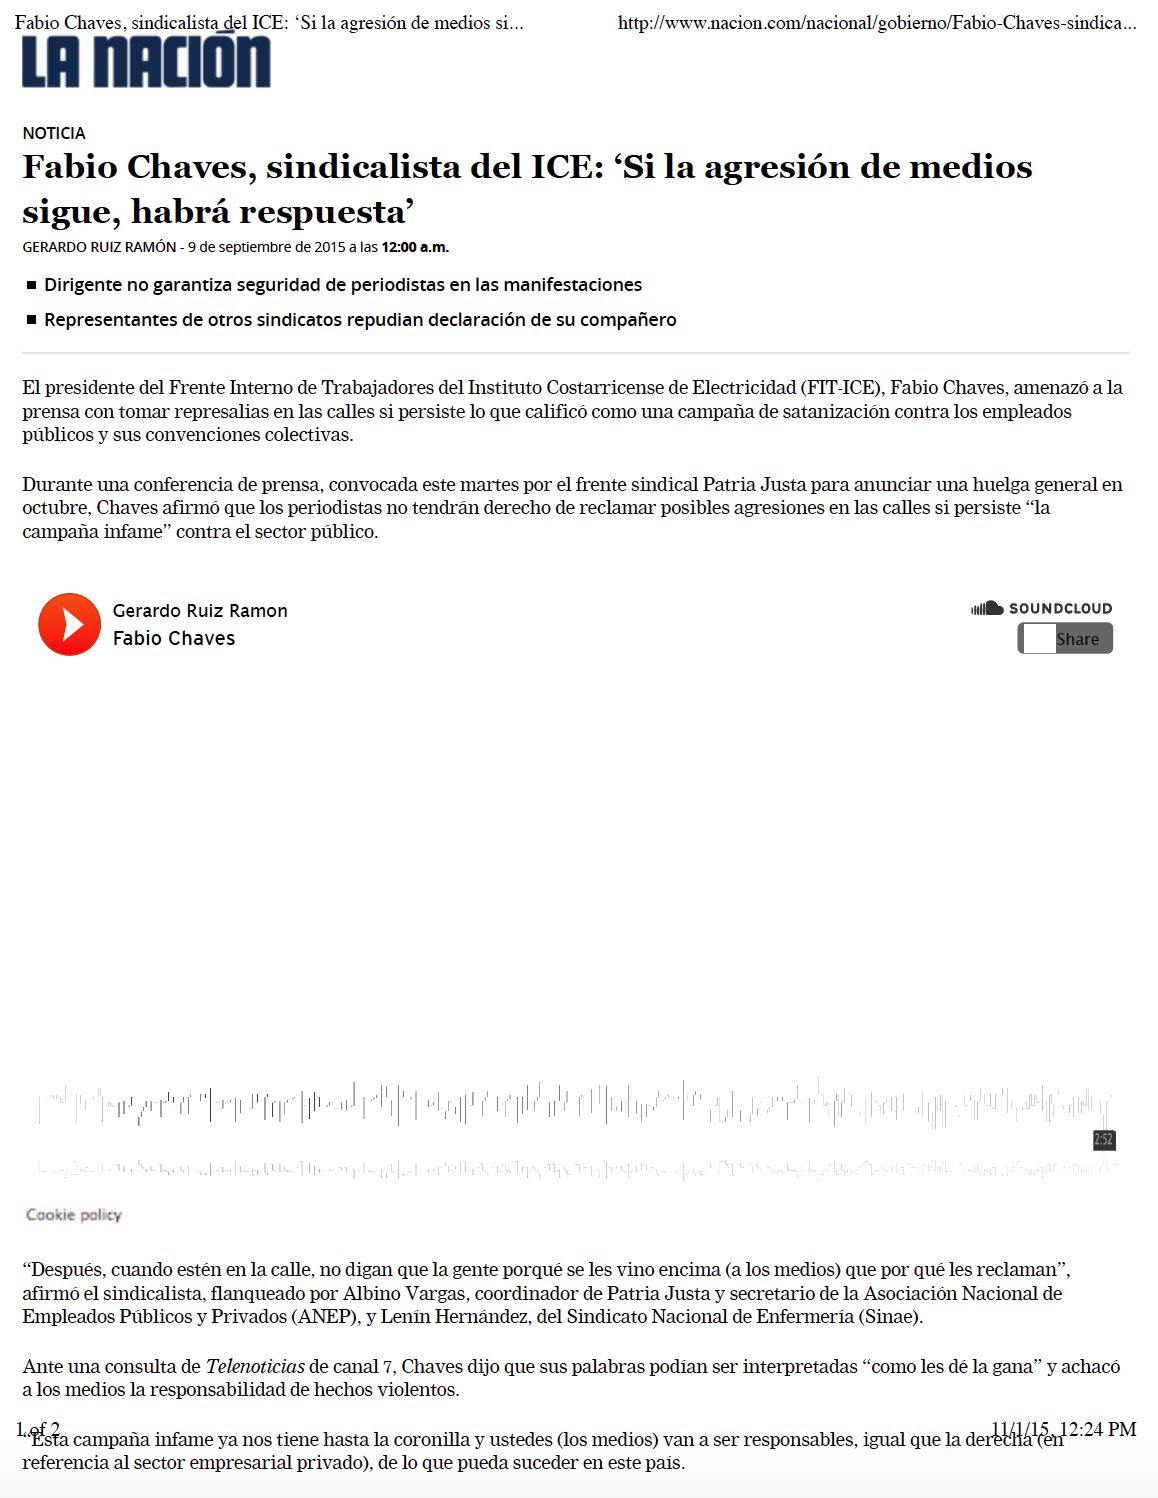
\includegraphics[width=15cm]{fabio-chaves-1}
    \captionof{figure}{Detalle de la noticia sobre el cuestionamiento del milagro de Floribeth Mora}
    \label{fig:falacia2}
\end{figure}

\begin{figure}[h!]
    \centering
    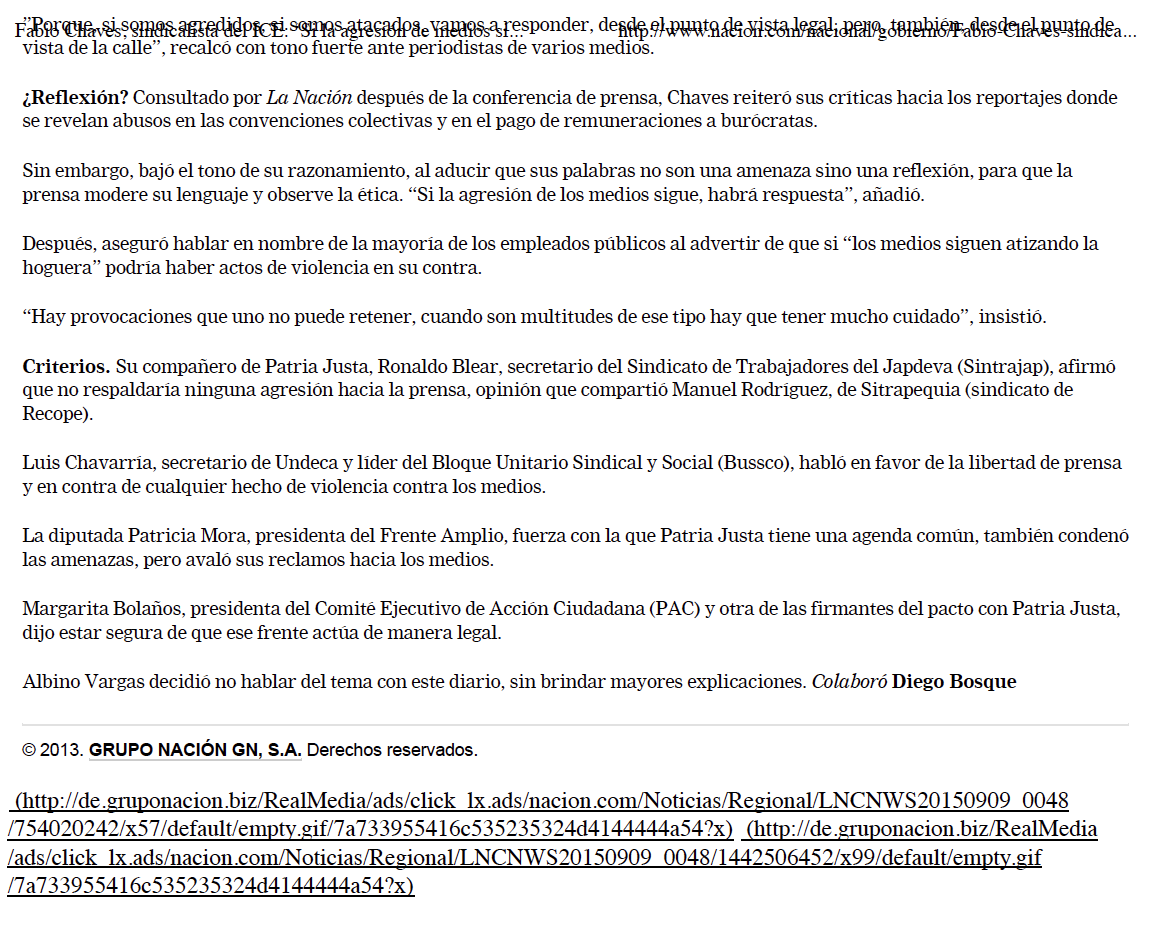
\includegraphics[width=15cm]{fabio-chaves-2}
    \captionof{figure}{Detalle de la noticia sobre el cuestionamiento del milagro de Floribeth Mora}
    \label{fig:falacia2}
\end{figure}

\newpage
\begin{table}[h!]
    \begin{tabular}{ll} 
        \toprule[1.5pt]
        Fuente & Periódico La Nación\\
        \midrule[0.5pt]
        Fecha  & 9 de setiembre 2015\\
        \midrule[0.5pt]
        Falacia & \textit{Ad Hominen} \\
        \bottomrule[1.5pt]
    \end{tabular} 
\end{table}

Durante este año la discusión acerca de los salarios y beneficios de los empleados públicos ha sido intensa. Medios de comunicación radiales, televisivos y escritos han dado mucho cobertura al respecto .
El día martes 8 de setiembre en conferencia de presa, el presidente del Frente Interno de Trabajadores del Instituto Costarricense de Electricidad, Fabio Chaves amenazó a la prensa y al público en general con tomar acciones si se continuaban haciendo denuncias hacia los empleados públicos.

Chaves llegó a decir: \textit{``Después, cuando estén en la calle, no digan que la gente porqué se les vino encima que por qué les reclaman''}, más adelante añadió: \textit{``Porque, si somos agredidos, si somos atacados, vamos a responder, desde el punto de vista legal, pero, también, desde el punto de vista de la calle''}.

Lo anterior, es un caso de falacia de tipo \textit{Ad Hominen}. Fabio Chaves se dedicó en atacar a los medios presentes en la conferencia y a desprestigiar sus posiciones a base de amenazas. Casi y que se podría llegar a interpretar que el sindicalista estaba haciendo más un llamado ``a las armas'' en lugar de una  llamado a una huelga y, tomando en cuenta que esto viene de un líder sindical, las consecuencias a este llamado pudieron haber llegado a ser muy fuertes. 

\section{Falacia 5: Lorem Ipsum}

\section{Falacia 6: Lorem Ipsum}

\section{Falacia 7: Lorem Ipsum}

\section{Falacia 8: Lorem Ipsum}

\section{Falacia 9: Lorem Ipsum}

\section{Falacia 10: Lorem Ipsum}

\section{Falacia 11: Lorem Ipsum}

\section{Falacia 12: Lorem Ipsum}


\begin{thebibliography}{9}

\bibitem{R1} Kopka~H, Daly~PW. 2003. \emph{A Guide to \LaTeX} (4th~edn).
Addison-Wesley.

\bibitem{R2} Lamport~L. 1994. \emph{\LaTeX: a Document Preparation System} (2nd~edn).
Addison-Wesley.

\bibitem{R3} Mittelbach~F, Goossens~M. 2004. \emph{The \LaTeX\ Companion}
(2nd~edn). Addison-Wesley.
\end{thebibliography}
\end{document}

